% !TEX root = ../msimplicial.tex

\section{Multisimplicial sets and geometric realization}

\anibal{say something here}

\subsection{Multisimplicial sets}

Let us consider an arbitrary non-negative integer~$k$.
The \textit{$k$-fold multisimplex category} $\msimplex{k}$ is the $k$-fold Cartesian product of the simplex category $\simplex$.
We denote the category of presheaves $\Fun((\msimplex{k})^\op, \Set)$ by $\mSet^{(k)}$ and refer to its objects as \textit{$k$-fold multisimplicial sets}.
The representable $k$-fold multisimplicial sets are denoted by
\[
\simplex^{n_1, \dots, n_k} = \yoneda \big( [n_1] \times \cdots \times [n_k] \big)
\]
and we have
\[
\simplex^{n_1, \dots, n_k} \big( [m_1] \times \cdots \times [m_k] \big) \cong
\simplex^{n_1}_{m_1} \times \dots \times \simplex^{n_k}_{m_k}.
\]
Explicitly, a $k$-fold multisimplicial set $X$ consists of a collection of sets
\[
X_{m_1, \dots, m_k} = X\big( [m_1] \times \cdots \times [m_k] \big)
\]
indexed by tuples of non-negative integers $(m_1, \dots, m_k)$ together with \textit{face maps}
\[
\face_i^j \colon
X_{m_1, \dots, m_j, \dots, m_k} \to
X_{m_1, \dots, m_j-1, \dots, m_k}
\]
and \textit{degeneracy map}
\[
\dege^j_i \colon X_{m_1, \dots, m_l, \dots, m_k} \to X_{m_1, \dots, m_j+1, \dots, m_k}
\]
for $1 \leq j \leq k$ and $0 \leq i \leq m_j$ such that, referring to $j$ as the \textit{direction} of these maps, two of them satisfy the simplicial identities when they have the same direction and commute when they do not.

The category of \textit{multisimplicial sets} is the coproduct
\[
\mSet = \coprod_{k \in \N} \mSet^{(k)}.
\]

\subsection{Diagonal simplicial set} \label{ss:diagonal simplicial set}

Precomposing with the diagonal functor
\[
\simplex^\op \xra{\diag}
(\simplex^\op)^{\times k} \xra{\cong}
(\msimplex{k})^{\op}
\]
defines a functor
\[
(-)^{\diag} \colon \mSet \to \sSet
\]
explicitly defined on a multisimplicial set $X$ by
\[
X^{\diag} \big( [n] \big) = X \big( [n] \times \dots \times [n] \big).
\]
It is straightforward to verify that
\[
\big( \simplex^{n_1, \dots, n_k} \big)^{\diag} \cong
\simplex^{n_1} \times \dots \times \simplex^{n_k}
\]
as simplicial sets.

This functor admits a right adjoint $\fM \colon \sSet \to \mSet$ which is defined on a simplicial set $Y$ by
\[
\fM(Y)_{m_1, \dots, m_k} =
\sSet\big( \simplex^{m_1} \times \dots \times \simplex^{m_k}, \, Y \big).
\]

%Although we do not use it in this work, we mention that $(-)^{\diag}$ and $\fM$ define a Quillen equivalence between simplicial and multisimplicial sets.

\subsection{Geometric realization}

The \textit{geometric realization} functor
\[
\bars{-} \colon \mSet \to \Top
\]
is defined as the Yoneda extension of the functor defined on representable objects by
\[
\bars{\simplex^{n_1, \dots, n_k}} =
\gsimplex^{n_1} \times \dots \times \gsimplex^{n_k}
\]
where we use the model
\[
\gsimplex^n = \big\{
(t_1, \dots, t_n) \in [0,1]^n \mid t_1 \geq \dots \geq t_n
\big\}
\]
with
\[
\delta_i(t_1, \dots, t_n) = \begin{cases}
(1, t_1, \dots, t_n) & i = 0, \\
(t_1, \dots, t_i, t_i, \dots, t_n) & 0 < i < n, \\
(1, t_1, \dots, t_n) & i = n,
\end{cases}
\]
and
\[
\sigma_i(t_1, \dots, t_n) = (t_1, \dots, \widehat t_i, \dots, t_n).
\]
Explicitly,
\[
\bars{X} =
\coprod X_{i_1,\dots,i_k} \times \gsimplex^{n_1} \times \dots \times \gsimplex^{n_k} /\sim
\]
where
\[
\begin{split}
(\face_i^j(x), t_1, \dots, t_j, \dots, t_k) &\sim (x, t_1, \dots, \delta_i(t_j), \dots, t_k), \\
(\dege^j_i(x), t_1, \dots, t_j, \dots, t_k) &\sim (x, t_1, \dots, \sigma_i(t_j), \dots, t_k).
\end{split}
\]

The restriction of the geometric realization functor to the subcategory of $1$-fold multisimplicial sets recovers the usual geometric realization of simplicial sets up to natural equivalence.

\subsection{Simplicial subdivision}

Consider the geometric realization $\gsimplex^{n_1} \times \dots \times \gsimplex^{n_k}$ of a representable multisimplicial set $\simplex^{n_1, \dots, n_k}$ and the geometric realization of its diagonal simplicial set $\bars{\simplex^{n_1} \times \dots \times \simplex^{n_k}}$.
The later can be thought of as a subdivision of the former with top dimensional cells in canonical bijection with $(n_1, \dots, n_k)$-shuffles.

This are ... \anibal{add}
The bijection is defined in analogy to \anibal{See Greg Friedman's appendix.}

We refer to the natural cellular map
\[
\ez \colon
\gsimplex^{n_1} \times \dots \times \gsimplex^{n_k} \to
\bars{\simplex^{n_1} \times \dots \times \simplex^{n_k}}
\]
as the \textit{Eilenberg--Zilber map}.

\subsection{Comparing $\bars{X}$ and $\bars{X^{\diag}}$}

Let $X$ be a multisimplicial set.
The natural composition
\begin{equation} \label{e:ez comparison}
\begin{split}
\bars{X} \ &\xra{\cong}
\colim_{(\simplex^{n_1, \dots, n_k} \downarrow X)} \bars{\simplex^{n_1, \dots, n_k}} \\ &\xra{=}
\colim_{(\simplex^{n_1, \dots, n_k} \downarrow X)} \gsimplex^{n_1} \times \dots \times \gsimplex^{n_k} \\ &\xra{\ez}
\colim_{(\simplex^{n_1, \dots, n_k} \downarrow X)} \bars{\simplex^{n_1} \times \dots \times \simplex^{n_k}} \\ &\xra{\cong}
\bars{X^{\diag}}
\end{split}
\end{equation}
is a cellular map whose underlying continuous map is a homeomorphism.
In fact, it can be thought of as the amalgamation map of a subdivision.
We refer to this extension of $\ez$ as \textit{Eilenberg--Zilber comparison} and use the same notation for it.

\anibal{Reference Quillen's proof.}

\subsection{Cartan--Serre map and the fundamental simplex}

The \textit{Cartan--Serre map} is the composition
\[
\cs \colon
\gsimplex^{n_1} \times \dots \times \gsimplex^{n_k} \to
[0,1]^{n_1 + \dots + n_k} \to
\gsimplex^{n_1 + \dots + n_k}
\]
where the first map is the canonical inclusion and the second is the projection defined by
\[
(x_1, \dots, x_{n_1 + \dots + n_k}) \mapsto (x_1, x_1x_2, \dots, x_1x_2 \dots x_{n_1 + \dots + n_k}).
\]

\anibal{This should induce a cellular homotopy inverse to the map in the previous section}

The image of the Cartan--Serre map is referred to as the \textit{fundamental simplex}. \anibal{Write this better.}

\subsection{Two important over-categories}

%The simplicial inclusions $\simplex^{n_1 + \dots + n_k} \to \simplex^{n_1} \times \dots \times \simplex^{n_k}$ are parameterized by \anibal{partitions and paths}, compare with the $\EZ$ map.
%We make a choice of a canonical such inclusion.
%The \textit{fundamental simplex} of $\simplex^{n_1} \times \dots \times \simplex^{n_k}$. \anibal{Choose one canonically}

In terms of shuffles, the fundamental simplex corresponds to \anibal{Andrea?}
So we have an inclusion of simplicial sets
\[
\simplex^n \to \simplex^{n_1} \times \dots \times \simplex^{n_k}
\]
These simplicial inclusions induce a functor
\[
\incl \colon (\simplex^{n_1} \times \dots \times \simplex^{n_k} \downarrow Y) \to (\simplex^n \downarrow Y)
\]
of over-categories in $\sSet$ for any simplicial set $Y$, which satisfies the following property.

\begin{lemma} \label{l:final functor}
	For all categories $\sC$ and all functors $F \colon (\simplex^n \downarrow Y) \to \sC$ the natural morphism between colimits
	\[
	\colim F \circ \incl \to \colim F
	\]
	is an isomorphism for any simplicial set $Y$.
\end{lemma}

\begin{proof}
	TBW
\end{proof}

\subsection{Comparing $\bars{\fM Y}$ and $\bars{Y}$}

Let $Y$ be a simplicial set.
We have a map
\[
\begin{split}
\bars{\fM Y} & \xra{\cong}
\colim_{(\simplex^{n_1, \dots, n_k} \downarrow \, \fM Y)} \gsimplex^{n_1} \times \cdots \times \gsimplex^{n_k} \\ & \xra{\cong}
\colim_{(\simplex^{n_1} \times \dots \times \simplex^{n_k} \downarrow \, Y)} \gsimplex^{n_1} \times \cdots \times \gsimplex^{n_k} \\ & \xra{\cs}
\colim_{(\simplex^{n_1} \times \dots \times \simplex^{n_k} \downarrow \, Y)} \gsimplex^{n_1 + \dots + n_k} \\ & \xra{\cong}
\colim_{(\simplex^{n} \downarrow \, Y)} \gsimplex^{n} \\ & \xra{\cong}
\bars{Y}
\end{split}
\]
where the third map is induced by regarding $\cs$ as a natural transformation and the fourth is defined by \cref{l:final functor}.

\anibal{make sure this map is a homotopy equivalence}

We refer to this natural cellular map as the \textit{Cartan--Serre comparison map}
\[
\cs \colon \bars{\fM Y} \to \bars{Y}.
\]

\subsection{Quillen equivalence}

\anibal{Reference or prove that $(-)^{\diag} \dashv \fM$ forms a Quillen equivalence.}

\section{Multisimplicial chains and algebraic structures}

\subsection{Chains}

The functor of \textit{chains} is the composition
\[
\chains \colon \mSet \xra{\bars{-}} \CW \xra{\gchains} \Ch
\]
of the geometric realization and functor of cellular chains.
It can also be described up to natural equivalence as the Yoneda extension of the functor defined on representable objects by
\[
\chains \big( \simplex^{n_1, \dots, n_k} \big) =
\chains(\simplex^{n_1}) \ot \dotsb \ot \chains(\simplex^{n_k}).
\]
Explicitly, \anibal{Add}

The functor of \textit{cochains} is defined using linear duality.

\subsection{Chain comparison maps} \label{ss:comparison chain maps}

Let $X$ be a multisimplicial set and $Y$ a simplicial set.
The Eilenberg--Zilber and Cartan--Serre comparison maps induce, by passing to cellular chains, natural quasi-isomorphism:
\[
\begin{split}
\ez &\colon \chains(X) \to \chains(X^{\diag}), \\
\cs &\colon \chains(\fM Y) \to \chains(Y), \\
\end{split}
\]
referred to as \textit{Eilenberg--Zilber} and \textit{Cartan--Serre comparison chain maps} respectively.
Notice that we are referring to the cellular map and its induced chain map by the same symbol.

\subsection{Counital coalgebras} \label{ss:coalgebras}

A \textit{counital coalgebra} consists of a chain complex $C$ and chain maps $\copr \colon C \to C \otimes C$ and $\aug \colon C \to \k$ satisfying
\[
(\id \otimes \aug) \circ \copr =
\id =
(\aug \otimes \copr) \circ \copr
\]
Denote by $\coAlg$ the category of coalgebras with morphisms being structure preserving chain maps.
The forgetful functor $\coAlg \to \Ch$ is symmetric monoidal with structure maps on $C \otimes C^\prime$ given by
\begin{gather*}
C \otimes C^\prime \xra{\copr \otimes \copr^\prime}
(C \otimes C) \otimes (C^\prime \otimes C^\prime) \xra{(23)}
(C \otimes C^\prime) \otimes (C \otimes C^\prime), \\
C \otimes C^\prime \xra{\aug \otimes \aug^\prime}
\k \otimes \k \xra{\cong} \k.
\end{gather*}

\subsection{Alexander--Whitney structure} \label{ss:alexander-whitney coalgebras}

Recall that $\chains(\simplex^n)$ is naturally a counital coalgebra with
\[
\begin{split}
\copr \big( [v_0, \dots, v_m] \big) &=
\sum_{i=0}^m \, [v_0, \dots, v_i] \ot [v_i, \dots, v_m], \\
\aug \big( [v_0, \dots, v_q] \big) &=
\begin{cases} 1 & \text{ if } q = 0, \\ 0 & \text{ if } q>0. \end{cases}
\end{split}
\]
Using the monoidal structure on $\coAlg$ we have natural coalgebra structures on
\[
\chains \big( \simplex^{n_1, \dots, n_k} \big) \cong
\chains(\simplex^{n_1}) \ot \dotsb \ot \chains(\simplex^{n_k})
\]
and therefore a natural counital coalgebra structure on any multisimplicial set $X$, which we refer to as the \textit{Alexander--Whitney structure}.

\anibal{Explicitly}

The product induced on cochains is referred to as \textit{multisimplicial cup product}.

\subsection{Coalgebra comparisons}

We now show that, with respect to the Alexander--Whitney coalgebra structures of \cref{ss:alexander-whitney coalgebras}, the Eilenberg--Zilber and Cartan--Serre comparison chain maps of \cref{ss:comparison chain maps} are quasi-isomorphisms of coalgebras.

\begin{theorem}
	For any multisimplicial set $X$
	\[
	\ez \colon \chains(X) \to \chains(X^{\diag})
	\]
	is a quasi-isomorphism of coalgebras.
\end{theorem}

\begin{proof}
	TBW \anibal{Formally follows from the Eilenberg--Zilber map inducing a coalgebra map}
\end{proof}

\begin{theorem}
	For any simplicial set $Y$
	\[
	\cs \colon \chains(\fM Y) \to \chains(Y)
	\]
	is a quasi-isomorphism of coalgebras.
\end{theorem}

\begin{proof}
	TBW \anibal{Formally follows from the Cartan--Serre map inducing a coalgebra map}
\end{proof}

\subsection{$\Med$-bialgebras}

An \textit{$\Med$-bialgebra} is a coalgebra $(C, \copr, \aug)$ together with a degree $1$ linear map $\pr \colon C \ot C \to C$, referred to as \textit{product}, whose boundary is $(\aug \ot \id) - (\id \ot \aug)$ and such that $\aug \circ \pr = 0$.
Let $\biAlg_\Med$ be the category of $\Med$-bialgebras with structure preserving morphisms.
The forgetful functor $\biAlg_\Med \to \coAlg$ is monoidal, with structure map on $C \otimes C^\prime$ given by
\[
(C \otimes C^\prime) \otimes (C \otimes C^\prime) \xra{(23)}
C \otimes C \otimes C^\prime \otimes C^\prime
\xra{\aug \otimes \id \otimes \pr + \pr \otimes \id \otimes \aug}
C \otimes C^\prime.
\]

\anibal{Flesh the $E_\infty$ stuff out}

As proven in \cite{medina2020prop1}, $\Med$-bialgebras are special cases of $E_\infty$-coalgebras.

\subsection{Multisimplicial join}

The \textit{join product} $\ast \colon \chains(\simplex^n)^{\ot 2} \to \chains(\simplex^n)$ is the natural degree~$1$ linear map defined by
\begin{multline}
\ast \big(\left[v_0, \dots, v_p \right] \ot \left[v_{p+1}, \dots, v_q\right]\big) = \\
\begin{cases} (-1)^{p} \sign(\pi) \left[v_{\pi(0)}, \dots, v_{\pi(q)}\right] & \text{ if } v_i \neq v_j \text{ for } i \neq j, \\
\hfil 0 & \text{ if not}, \end{cases}
\end{multline}
where $\pi$ is the permutation that orders the vertices.
It is an algebraic version of the usual join of faces in a simplex, please consult \cref{f:join of faces} for an example.

The Alexander--Whitney coalgebra structure together with the join product define a natural $\Med$-bialgebra structure on $\chains(\simplex^n)$. This extends monoidally to a natural $\Med$-bialgebra structure on
\[
\chains(\simplex^{n_1, \dots, n_k}) \cong
\chains(\simplex^{n_1}) \ot \dotsb \ot \chains(\simplex^{n_k}).
\]

\begin{figure}
	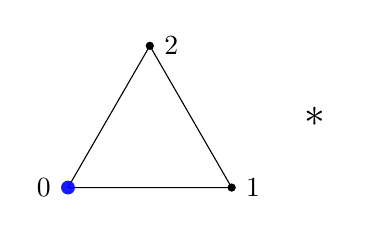
\begin{tikzpicture}[scale=.6]
\coordinate (A) at (210:2);
\coordinate (B) at (-30:2);
\coordinate (C) at (90:2);

\draw[draw=black] (A) -- (B) -- (C) -- (A);

\node[circle,fill=blue, opacity=.9, inner sep=0pt,minimum size=5pt, label=left:{0}] (a) at (A) {};
\node[circle,fill=black,inner sep=0pt,minimum size=3pt, label=right:{$1$}] (a) at (B) {};
\node[circle,fill=black,inner sep=0pt,minimum size=3pt, label=right:{$2$}] (a) at (C) {};

\node[scale=1.5] at (3.5,0.5) {$\ast$};
\end{tikzpicture}
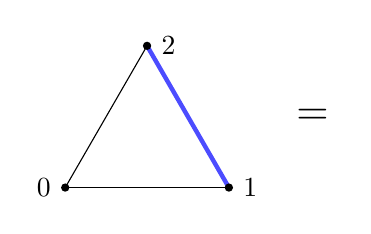
\begin{tikzpicture}[scale=.6]
\coordinate (A) at (210:2);
\coordinate (B) at (-30:2);
\coordinate (C) at (90:2);

\draw[draw=blue, ultra thick, draw opacity=.7] (B) -- (C);
\draw[draw=black] (C) -- (A);
\draw[draw=black] (A) -- (B);

\node[circle,fill=black,inner sep=0pt,minimum size=3pt, label=left:{$0$}] (a) at (A) {};
\node[circle,fill=black,inner sep=0pt,minimum size=3pt, label=right:{$1$}] (a) at (B) {};
\node[circle,fill=black,inner sep=0pt,minimum size=3pt, label=right:{$2$}] (a) at (C) {};

\node[scale=1.5] at (3.5,.5) {=};
\end{tikzpicture}
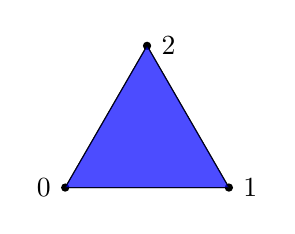
\begin{tikzpicture}[scale=.6]
\coordinate (A) at (210:2);
\coordinate (B) at (-30:2);
\coordinate (C) at (90:2);

\draw[draw=black] (A) -- (B) -- (C) -- (A);

\node[circle,fill=black,inner sep=0pt,minimum size=3pt, label=left:{$0$}] (a) at (A) {};
\node[circle,fill=black,inner sep=0pt,minimum size=3pt, label=right:{$1$}] (a) at (B) {};
\node[circle,fill=black,inner sep=0pt,minimum size=3pt, label=right:{$2$}] (a) at (C) {};

\draw[draw, fill=blue, opacity=.7] (A) -- (B) -- (C) -- (A);
\end{tikzpicture}
	\caption{Geometric representation of the join product of two basis elements. It depicts the identity $\pr \big( [0] \otimes [1,2] \big) = [0,1,2]$.}
	\label{f:join of faces}
\end{figure}